\documentclass{article}
\title{M1J2 Summary Notes (JMC Year 1, 2017/2018 syllabus)}
\date{}
\author{Fawaz Shah (original notes by Dr Marie-Amelie Lawn)}

% Packages for adding hyperlinks to table of contents
\usepackage{color}   %May be necessary if you want to color links
\usepackage{hyperref}
\hypersetup{
    colorlinks=true, %set true if you want colored links
    linktoc=all,     %set to all if you want both sections and subsections linked
    linkcolor=black,  %choose some color if you want links to stand out
}

%package that allows aligned equations
\usepackage{amsmath}

%package that allows notation for extra mathematical symbols
\usepackage{amssymb}

%new commands for popular sets for ease of use
\newcommand{\R}{\mathbb{R}}
\newcommand{\N}{\mathbb{N}}
\newcommand{\Z}{\mathbb{Z}}

% renaming command to writing vectors in bold notation
\renewcommand{\vec}[1]{\mathbf{#1}}

%package for managing images
\usepackage{graphicx}
\graphicspath{ {img/} }

%package for managing hyperlinks
\usepackage{hyperref}

%package for added blue colored boxes
\usepackage{tcolorbox}

%package that allowed removing indent from enumerate environment
\usepackage{enumitem}

\begin{document}
\large
\maketitle
\noindent (Dr Lawn refers to propositions, theorems, corollaries and lemmas. In this document I will refer to them all as 'theorems'.)
\\\\
This document contains a list of definitions and a list of theorems.
\\\\
Note that the exam will probably require you to PROVE some of these theorems, so you should refer back to the original notes for the proofs.
\\\\
Boxes cover content in more detail.
\tableofcontents
\newpage
\part{Abstract Linear Algebra}

\section{Definitions}
\paragraph{Vector space}
A vector space is a set $ V $ coupled with:
\begin{itemize}
\item a function $ + : V \times V \to V $ (addition)
\item a function $ \cdot : \R \times V \to V $ (scalar multiplication)
\end{itemize}
(For the rest of this part, we will assume $ V $ is a vector space)
\paragraph{Subspace}
A subset $ U \subseteq V $ is a subspace if:
\begin{itemize}
\item $ \vec{0}_{V} \in U $
\item If $ \vec{x}, \vec{y} \in U $ then $ \vec{x + y} \in U $ (closure under addition)
\item If $ \vec{x} \in U $ then for all $ \lambda \in \R $, $ \lambda\vec{x} \in U $ (closure under scalar multiplication)
\end{itemize}
\paragraph{Linear combination}
A linear combination of a set of vectors $ \{\vec{v}_{1}...\vec{v}_{n}\} $ is any vector $ \vec{x} $ of the form:
\begin{equation}
\vec{x} = \lambda_{1}\vec{v}_{1} + \lambda_{2}\vec{v}_{2} + ... + \lambda_{n}\vec{v}_{n}
\end{equation}
for some real numbers $ \lambda_{1}...\lambda_{n} $
\paragraph{Span}
The span of a set $ S \subseteq V $ is the set of all linear combinations of elements of $ S $. We define span$ (\emptyset) = \{\vec{0}_{V}\} $.
\paragraph{Spanning set}
A subset $ S \subseteq V $ is called a spanning set of $ V $ if span$ (S) = V $.
\paragraph{Linear dependence}
A subset of vectors $ \{ \vec{v}_{1}...\vec{v}_{n} \}  \subseteq V $ is linearly dependent if there exists some real numbers $ \lambda_{1}...\lambda_{n} $ (which are not just all $ 0 $s) such that:
\begin{equation}
\lambda_{1}\vec{v}_{1} + \lambda_{2}\vec{v}_{2} + ... + \lambda_{n}\vec{v}_{n} = \vec{0}_{V}
\end{equation}
\paragraph{Basis}
A basis of a vector space is a linearly independent spanning set.
\\\\
We can also think of a basis as a spanning set of minimum possible size, or a linearly independent set of maximum possible size (theorems to show this later).
\paragraph{Standard basis of $ \R^{n} $}
We define the standard basis elements of any $ \R^{n} $ to be:
\begin{equation}
e_{1} = 
\begin{pmatrix}
1 \\ 0 \\ \vdots \\ 0 \\ 0
\end{pmatrix} , \ 
e_{2} = 
\begin{pmatrix}
0 \\ 1 \\ \vdots \\ 0 \\ 0
\end{pmatrix} ... \
e_{n-1} = 
\begin{pmatrix}
0 \\ 0 \\ \vdots \\ 1 \\ 0
\end{pmatrix} , \
e_{n} = 
\begin{pmatrix}
0 \\ 0 \\ \vdots \\ 0 \\ 1
\end{pmatrix}
\end{equation}
The standard basis of $ \R^{n} $ is therefore $ \{e_{1}, e_{2} \ ... \ e_{n} \} $.
\paragraph{Dimension}
The dimension of a vector space is the size of any basis of that vector space.
\paragraph{Linear map}
Let $ U $ and $ V $ be vector spaces. A linear map is a function $ f : U \to V $ such that:
\begin{itemize}
\item for all $ \vec{x}, \vec{y} \in U, \ f(\vec{x} + \vec{y}) = f(\vec{x}) + f(\vec{y}) $
\item for all $ \vec{x} \in U $ and $ \lambda \in \R, \ f(\lambda \vec{x}) = \lambda f(\vec{x}) $
\end{itemize}
\paragraph{Image}
The image of a linear map $ f : U \to V $ is the set of all $ f(\vec{u}) \in V $ where $ \vec{u} \in U $.
\begin{equation}
\textrm{image}(f) = \{f(\vec{u}) \ | \ u \in U \}
\end{equation}
\paragraph{Kernel}
The kernel of a linear map $ f : U \to V $ is the set of all $ \vec{u} \in U $ such that $ f(\vec{u}) = \vec{0}_{V} $.
\begin{equation}
\textrm{kernel}(f) = \{\vec{u} \ | \ u \in U, f(\vec{u}) = \vec{0}_{V} \}
\end{equation}
\paragraph{Isomorphism}
A linear map $ f : U \to V $ is an isomorphism if it is bijective. We say $ U \simeq V $.
\paragraph{Rank}
The rank of $ f $ is defined as dim(image($ f $)).
\paragraph{Nullity}
The rank of $ f $ is defined as dim(kernel($ f $)).
\paragraph{$ T_{A} $}
We define a function $ T_{A} $ that pre-multiplies a vector by a matrix $ \vec{A} $:
\begin{equation}
T_{A} : \R^{n} \to \R^{m}, \ \vec{v} \mapsto \vec{A}\vec{v}, \ \vec{A} \in \textrm{Mat}_{m \times n}(\R)
\end{equation}
where $  \textrm{Mat}_{m \times n}(\R)  $ denotes the set of all $ m \times n $ matrices with real entries.
\\
Note that if $ \vec{A} $ is an $ m \times n $ matrix, then $ T_{A} $ transforms a vector in $ \R^{n} $ to a vector in $ \R^{m} $.
\paragraph{Matrix representing $ f $}
Following from the previous definition, if we have:
\begin{itemize}
\item $ B $ is a basis of $ U $
\item $ C $ is a basis of $ V $
\item There is an isomorphism $ f_{B} : \R^{n} \to U $
\item There is an isomorphism $ f_{C} : \R^{m} \to V $
\end{itemize}
We say the matrix $ \vec{A} $ is called the matrix representing $ f $ with respect to $ B $ and $ C $. This is denoted by:
\begin{equation}
\vec{A} =
\begin{bmatrix}
f
\end{bmatrix}_{B}^{C}
\end{equation}
\paragraph{Change-of-basis matrix}
Let $ B $ and $ C $ be two bases for $ V $. The matrix:
\begin{equation}
\vec{A} =
\begin{bmatrix}
\textrm{Id}_{V}
\end{bmatrix}_{B}^{C}
\end{equation}
is called the change-of-basis matrix from $ B $ to $ C $. $ \textrm{Id}_{V} $ denotes the identity function in the vector space $ V $ (maps every vector to itself).
\\\\
In this case the linear map $ T_{A} $ will convert a vector given with respect to the basis $ B $ into a vector with respect to the basis $ C $.
\paragraph{'Vector with respect to a basis'}
If we have an $ n $-dimensional vector space $ V $ and a basis $ B = \{\vec{b}_{1} ... \vec{b}_{n} \} $, then we say any $ \vec{v} \in V $  is given with respect to $ B $ if:
\begin{equation}
\vec{v} = 
\begin{pmatrix}
\lambda_{1} \\ \lambda_{2} \\ \vdots \\ \lambda_{n}
\end{pmatrix} , \ 
\vec{v} = \lambda_{1}\vec{b}_{1} + \lambda_{2}\vec{b}_{2} + ... + \lambda_{n}\vec{b}_{n}
\end{equation}

\section{Theorems}

\subsection{Vector spaces}
\textit{Vector space axioms}
\begin{itemize}
\item $ (V, +) $ is an Abelian group (the identity element being $ \vec{0}_{V} $)
\item for any $ \vec{v} \in V $, 1$ \vec{v} = \vec{v} $
\item for any $ \vec{v} \in V, \lambda, \mu \in \R, \lambda (\mu \vec{v}) = (\lambda \mu) \vec{v} $ (commutative w.r.t. scalar multiplication)
\item for any $ \vec{u}, \vec{v} \in V, \lambda \in \R, \lambda (\vec{u}  + \vec{v}) = \lambda \vec{u}  + \lambda \vec{v} $ (scalar multiplication distributes over addition)
\item for any $ \vec{v} \in V, \lambda, \mu \in \R, (\lambda + \mu) \vec{v} = \lambda \vec{v}  + \mu \vec{v} $ (scalar multiplication distributes over scalar addition)
\end{itemize}
For any $ \vec{v} \in V $:
\begin{itemize}
\item For any $ n \in \Z $, $ n\vec{v} = \vec{v} + \vec{v} + ... + \vec{v} $ (n times)
\item $ 0 \vec{v} = \vec{0}_{V} $
\item $ (-1) \vec{v} $ is the additive inverse of $ \vec{v} $
\end{itemize}

\subsection{Subspaces}
Every vector space $ V $ has two trivial subspaces, itself and $ \{ \vec{0}_{V} \} $.
\\\\
For any subspaces $ U, W \subseteq V $:
\begin{itemize}
\item $ U \cap W $ is a subspace
\item $ U \cup W $ is NOT a subspace
\end{itemize}
Any $ U \subseteq V $ is a subspace iff every linear combination of vectors in $ U $ is again in $ U $ (i.e. $ \textrm{span}(U) \subseteq U $).
\\\\
For any $ S \subseteq V $, span$ (S) $ is a subspace.
\\\\
If $ U  \subset V $ is a subspace and $ S \subset U $ then span$ (S) \subset U $.

\subsection{Spanning sets, linear independence, bases, dimension}
Every element of a vector space $ V $ can be written as a unique linear combination of basis vectors (for any basis).
\\\\
For any set $ S \subseteq V $:
\begin{itemize}
\item If $ \vec{v}_{1} = \lambda\vec{v}_{2} $ for any $ \vec{v}_{1}, \vec{v}_{2} \in S $ then $ S $ is linearly dependent
\item If $ \vec{0}_{V} \in S $ then $ S $ is linearly dependent
\end{itemize}
If a set $ S $ is linearly independent/dependent then any subset of $ S $ is also linearly independent/dependent respectively.
\\\\
A vector space is finite dimensional if it contains a finite spanning set.
\\\\
Every finite spanning set contains a basis.
\\\\
Therefore, a vector space is finite dimensional if it has a finite basis.
\\\\
If a finite dimensional vector space has a basis, then there exists a finite dimensional spanning set.
\\\\
If $ S \subseteq V $ is a linearly DEPENDENT spanning set, there exists some $ \vec{s} \in S $ such that $ S - \{\vec{s}\} $ is still a spanning set.
\begin{tcolorbox}
In other words, we can keep removing elements from a spanning set until it is linearly independent. At this point the spanning set is now a basis, by definition. This gives us our alternate definition of a basis as a spanning set of minimum size.
\end{tcolorbox}
\noindent
\\
\textit{Steinitz exchange lemma - base case}
\\
Let $ S \subset V $ be a spanning set, and let $ \vec{v} \in V $. There always exists an $ \vec{s} \in S $ such that
\begin{equation}
(S \setminus \{\vec{s}\}) \cup \{\vec{v}\}
\end{equation}
is still a spanning set.
\\\\
\textit{Steinitz exchange lemma - in full}
\\
Let $ S \subset V $ be a spanning set, and let $ \vec{v}_{1}...\vec{v}_{n} \in V $ be a linearly independent set. There always exists some $ \vec{s}_{1}...\vec{s}_{n} \in S $ such that
\begin{equation}
(S \setminus \{\vec{s}_{1}...\vec{s}_{n}\}) \cup \{\vec{v}_{1}...\vec{v}_{n}\}
\end{equation}
is still a spanning set.
\begin{tcolorbox}
In other words, we can substitute in any linearly independent set, and $ S $ will still be a spanning set.
\end{tcolorbox}
\noindent
\\
Any linearly independent set is smaller than or equal to any spanning set. (Consequence of Steinitz exchange lemma).
\\\\
If $ L \subset V $ linearly independent and $ \vec{v} \notin \textrm{span}(L) $ then $ L \cup {\vec{v}} $ is linearly independent.
\begin{tcolorbox}
In other words, we can keep adding elements to a linearly independent set until it is a spanning set. At this point the linearly independent set is a basis, by definition. This gives us our alternate definition of a basis as a linearly independent set of maximum size.
\end{tcolorbox}
\noindent
\\
If $ \dim(V) = n $ then every basis of $ V $ has size $ n $.
\\\\
If $ V $ is infinite-dimensional, we can always find a linearly independent subset of $ V $ with size $ n $, for any $ n $.
\\\\
Any linearly independent set is contained in a basis.
\\\\
Any linearly independent set $ L $ where $ \#L = \dim(V) $ is a basis.
\\\\
If $ V $ is finite dimensional and $ U \in V $:
\begin{itemize}
\item $ U $ is finite dimensional
\item $ \dim(U) \leq \dim(V) $
\item if $ \dim(U) = \dim(V) $ then $ U = V $
\end{itemize}

\subsection{Linear maps}
(For the rest of this subsection assume $ f, g $ are linear maps, and let $ f : U \to V $)
\\\\
$ g \circ f $ is also a linear map.
\\\\
$ f(\vec{0}_{U}) = f(\vec{0}_{V}) $.
\\\\
$ \textrm{image}(f) $ is a subspace of $ V $.
\\
$ \textrm{kernel}(f) $ is a subspace of $ U $.
\\\\
If $ f $ surjective then $ \textrm{image}(f) = V $.
\\
If $ f $ injective then $ \textrm{kernel}(f) = \{\vec{0}_{U}\} $.
\\\\
If $ f(\vec{x}) = \vec{y} $ then $ f^{-1}(\vec{y}) = \{\vec{x} + \vec{w} \ | \ \vec{w} \in \textrm{kernel}(f) \} $.
\\\\
If $ f : \R^{n} \to \R^{m} $ then $ f \equiv T_{A} $ for some matrix $ \vec{A}  \in \textrm{Mat}_{m \times n}(\R) $.
\begin{tcolorbox}
Specifically $ f : \lambda_{1}\vec{e}_{1} + ... + \lambda_{n}\vec{e}_{n} \mapsto \lambda_{1}f(\vec{e}_{1}) + ... + \lambda_{n}f(\vec{e}_{n}) $
\\\\
Therefore we can set:
\begin{equation}
\vec{A} = [f(\vec{e}_{1}) \ | \ f(\vec{e}_{2}) \ | \ ... \ |\  f(\vec{e}_{n})]
\end{equation}
so that for any $ \vec{v} \in U $:
\begin{equation}
T_{A}(\vec{v}) = \vec{A}
\begin{bmatrix}
\lambda_{1} \\ \lambda_{2} \\ \vdots \\ \lambda_{n}
\end{bmatrix}
= \lambda_{1}f(\vec{e}_{1}) + ... + \lambda_{n}f(\vec{e}_{n})
\end{equation}
\end{tcolorbox}
\noindent
\\
Let $ g : U \to V $, let $ B = \{\vec{b}_{1}...\vec{b}_{n}\} $ be a basis of $ U $.
\\
If $ f(\vec{b}_{i}) = g(\vec{b}_{i}) $ for all $ \vec{b}_{i} $ then $ f \equiv g $.
\\\\
There is always a linear map between a basis of $ U $ and any set of vectors in $ V $.
\\\\
If $ U \simeq V $ then $ \dim(U) = \dim(V) $
\\\\
If $ \dim(V) = n $ then $ f \simeq \R^{n} $.
\\\\
Let $ B = \{\vec{b}_{1}...\vec{b}_{n}\} $ be a basis of $ U $ and $ C = \{f(\vec{b}_{1})...f(\vec{b}_{n})\} $ a subset of $ V $:
\begin{itemize}
\item $ \textrm{span}(C) = \textrm{image}(f) $
\item $ C $ is a spanning set $ \Leftrightarrow f $ is surjective
\item $ C $ is linearly independent $ \Leftrightarrow f $ is injective
\item $ C $ is a basis $ \Leftrightarrow f $ is bijective (aka an isomorphism)
\end{itemize}
If $ \dim(U) = \dim(V) $ then $ f \textrm{ bijective} \Leftrightarrow f \textrm{ surjective} \Leftrightarrow f \textrm{ injective} $
\\\\
\textit{Rank-Nullity Theorem}
\\
$ \textrm{rank}(f) + \textrm{nullity}(f) = \dim(U) $
\\\\
Any $ f : U \to V $ can be represented as $ T_{A} $ for some matrix $ \vec{A} $.
\begin{tcolorbox}
\textit{Steps for computing $ \vec{A} $:}
\\\\
Let $ B = \{\vec{b}_{1}...\vec{b}_{n}\} $ be a basis of $ U $
\\
Let $ C = \{\vec{c}_{1}...\vec{c}_{m}\} $ be a basis of $ V $
\\\\
We have isomorphisms:
\\
$ f_{B} : \R^{n} \to U, \ \lambda_{1}\vec{e}_{1} + ... + \lambda_{n}\vec{e}_{n} \mapsto \lambda_{1}\vec{b}_{1} + ... + \lambda_{n}\vec{b}_{n} $
\\
$ f_{C} : \R^{m} \to V, \ \lambda_{1}\vec{e}_{1} + ... + \lambda_{m}\vec{e}_{m} \mapsto \lambda_{1}\vec{c}_{1} + ... + \lambda_{m}\vec{c}_{m} $
\\\\
Note that the linear map $ (f_{C})^{-1} \circ f \circ f_{B} $ sends vectors from $ \R^{n} \to \R^{m} $, therefore we can define:
\begin{equation}
T_{A} \equiv (f_{C})^{-1} \circ f \circ f_{B}
\end{equation}
since, from earlier, $ T_{A} : \R^{n} \to \R^{m} $.
\begin{enumerate}[leftmargin=*]
\item Take basis vectors of $ U $ ($ \vec{b}_{j} $) in some order. Compute $ f(\vec{b}_{j}) $. We have just applied $ f_{B} $, followed by $ f $.
\item Express each $ f(\vec{b}_{j}) $ as a linear combination of basis vectors of $ V $ ($ \vec{c}_{i} $).
\item Applying $ (f_{C})^{-1} $ sends vectors in $ V $ to their coefficients w.r.t the basis vectors $ \vec{c}_{i} $.
\end{enumerate}
The matrix $ A $ is such that the $ j^{th} $ column of $ A $ is the vector $ (f_{C})^{-1} \circ f \circ f_{B}(\vec{e}_{j})  = (f_{C})^{-1} \circ f(\vec{b}_{j}) $
\end{tcolorbox}

\newpage
\part{Group Theory}

\section{Definitions}
\paragraph{Binary operation}
A binary operation on a set $ G $ is a any function $ f: G \times G \to G $
\paragraph{Associative}
A binary operation $ \star $ on a set $ G $ is associative if it satisfies:
\begin{equation}
(a \star b) \star c = a \star (b \star c)
\end{equation}
for all $ a, b, c \in G $.
\paragraph{Commutative}
A binary operation $ \star $ on a set $ G $ is commutative if it satisfies:
\begin{equation}
a \star b = b \star a
\end{equation}
for all $ a, b \in G $.
\paragraph{Left/right identity}
An element $ e \in G $ is called the left identity if:
\begin{equation}
e \star g = g
\end{equation}
for all $ g \in G $. Similar statement for right identity.
\paragraph{(Two sided) Identity element}
An element $ e \in G $ is a two-sided identity element if it is both a left identity and a right identity.
\\\\
From now on the two-sided identity element will be referred to as $ e $.
\paragraph{Left/right inverse}
An element $ h \in G $ is called the left inverse  of $ g \in G $ if:
\begin{equation}
h \star g = e
\end{equation}
Similar statement for right inverse.
\paragraph{Two sided inverse}
A two sided inverse of an element $ g \in G $ is both a left inverse and a right inverse of $ g $.
\\\\
From now on the two-sided inverse of $ g $ will be referred to as $ g^{-1} $.
\paragraph{Group}
A group $ (G, \star) $ is a set $ G $ equipped with a binary operation $ \star $ such that:
\begin{itemize}
\item $ \star $ is associative
\item $ \star $ has an identity element $ e \in G $
\item Every $ g \in G $ has an inverse $ g^{-1} \in G $
\end{itemize}
\begin{tcolorbox}
The above three suffice for the exam, however there is technically a fourth requirement:
\begin{itemize}
\item $ G $ is closed under $ \star $, i.e. for all $ g, h, \in G, g \star h \in G $
\end{itemize}
\end{tcolorbox}
(For the rest of this part, we will assume $ (G, \star) $ is a group)
\paragraph{Order (group)}
The order of a group $ (G, \star) $ is the size of $ G $.
\paragraph{Abelian group}
An Abelian group is a group with a commutative binary operation $ \star $.
\paragraph{Powers of $ g $}
We can define the powers of any $ g \in G $ to be:
\begin{equation}
g^{n} = 
\begin{cases}
g \star g \star ... g & n > 0 \\
g^{-1} \star g^{-1} \star ... g^{-1} & n < 0 \\
e & n = 0
\end{cases}
\end{equation}
where in the first cases there are $ n $ copies of $ g $, and in the second case there are $ -n $ copies of $ g^{-1} $.
\paragraph{Definition of $ [a]_{n} $ and $ \Z_{n} $}
For any $ a \in \Z $:
\begin{equation}
[a]_{n} = \{b \in \Z \ | \ b \equiv a \textrm{ mod } n \}
\end{equation}
Note that $ [a]_{n} $ forms an equivalence class, and there are exactly $ n $ of these equivalence classes. $ \Z_{n} $ is the set of all these equivalence classes.
\begin{equation}
\Z_{n} = \{[a]_{n} \ | \ a \in \Z \}
\end{equation}
\paragraph{Definition of $ \Z_{n}^{*} $}
$ \Z_{n}^{*} $ is the set of all invertible $ [a]_{n} $. Note in this case the identity element is $ [1]_{n} $.
\begin{equation}
\Z_{n}^{*} = \{[a]_{n} \ | \ \exists [b]_{n} \in Z_{n} \quad s.t. \quad [a]_{n}[b]_{n} = [1]\}
\end{equation}
Note that $ [a]_{n}[b]_{n} = 1 \Leftrightarrow gcd(a, n) = 1 $.
\paragraph{Order (element)}
The order of any $ g \in G $ is the smallest positive integer such that:
\begin{equation}
g^{n} = e
\end{equation}
\paragraph{Cyclic group + generator}
A group $ (G, \star) $ is cyclic if:
\begin{equation}
G = \{ g^{n} \ | \ n \in \Z \} 
\end{equation}
$ g $ is called the generator of the group.
\paragraph{Permutation}
A permutation $ \sigma $ on $ n $ symbols is a bijection:
\begin{equation}
\sigma : \{1...n\} \to \{1...n\}
\end{equation}
\paragraph{Symmetric group}
The symmetric group $ S_{n} $ on $ n $ symbols is the set of all permutations of $ n $ symbols.
\begin{equation}
S_{n} = \{\sigma : \{1...n\} \to \{1...n\}\}
\end{equation}
Note that $ S_{n} $ is a set of functions. Therefore the identity element is the identity function.
\paragraph{$ k $-cycle}
A permutation $ \sigma \in S_{n} $ is a $ k $-cycle if there exists some $ a_{1}...a{k}  \in \{1...n\} $ such that:
\begin{equation}
\sigma(a_{1}) = a_{2}, \quad \sigma(a_{2}) = a_{3} \quad ... \quad \sigma(a_{k}) = a_{1}
\end{equation}
and $ \sigma(i) = i $ for all $ i \notin \{1...n\} $. $ k $ is called the length of the cycle. The notation for a cycle is $ (a_{1}...a_{k}) $.
\paragraph{Disjoint cycles}
Two cycles $ (a_{1}...a_{m}) $ and $ (b_{1}...b_{n}) $ are disjoint if no $ a_{i} $ is equal to any $ b_{j} $.
\paragraph{Subgroup}
Let $ (G, \star) $ be a group, and $ H \subseteq G $. $ (H, \star) $ is a subgroup of $ G $ if:
\begin{itemize}
\item $ e \in H $
\item For any $ g, h \in H $,  $ g \star h \in H $
\item For any $ g \in H $, $ g^{-1} \in H $
\end{itemize}
\paragraph{Cyclic subgroup}
Let $ (G, \star) $ be a group. For any $ g \in G $, the cyclic subgroup $ \langle g \rangle $ generated by $ g $ is defined as:
\begin{equation}
\langle g \rangle = (\{g^{i} \ | \ i \in \Z \}, \star)
\end{equation}
Note that order of $ g  = $  size of cyclic subgroup $ \langle g \rangle $.
\paragraph{Left/right cosets}
Let $ (G, \star) $ be a group and $ (H, \star) $ a subgroup. For any $ g \in G $, the left coset of $ H $ by $ g $ (denoted by $ gH $) is defined as:
\begin{equation}
gH = \{g \star h \ | \ h \in H \}
\end{equation}
Similar definition for right coset of $ H $ by $ g $ (denoted by $ Hg $).
\\\\
The set of all left cosets of $ H $ by $ g $ is denoted by $ G : H $.
\\
The set of all right cosets of $ H $ by $ g $ is denoted by $ H : G $.

\section{Theorems}

\subsection{Groups}
Any identity element $ e $ is unique for that group.
\\\\
Any two-sided inverse $ g^{-1} $ of an element $ g \in G $ is unique.
\\\\
For any $g, h \in G $
\begin{equation}
(g \star h)^{-1} = h^{-1} \star g^{-1}
\end{equation}
The normal exponent rules apply within groups, e.g.
\begin{align}
g^{n} \star g^{m} & = g^{n+m} \\
(g^{n})^{-1} & = g^{-n} \\
(g^{n})^{m} & = g^{nm}
\end{align}
Some examples of groups:
($ \R, + $), ($ \Z, + $), ($ \Z^{*}, \times $)


\subsection{Modular arithmetic and $ \Z_{n} $}
($ \Z_{n}, + $) is an Abelian group.
\\\\
($ \Z_{n}^{*}, \ \cdot \ $) is an Abelian group.

\subsection{Cyclic groups}
If ($ G, \star $) is a finite group then every $ g \in G $ has finite order.
\\\\
Any $ g \in G $ with order n has distinct powers $ g^{0}, g^{1}, g^{2}...g^{n - 1} $.
\\\\
All cyclic groups are Abelian.
\\\\
Assume $ G $ is finite with size $ n $. \\
$ G $ is cyclic $ \Leftrightarrow G $ contains an element of order $ n $.
\\\\
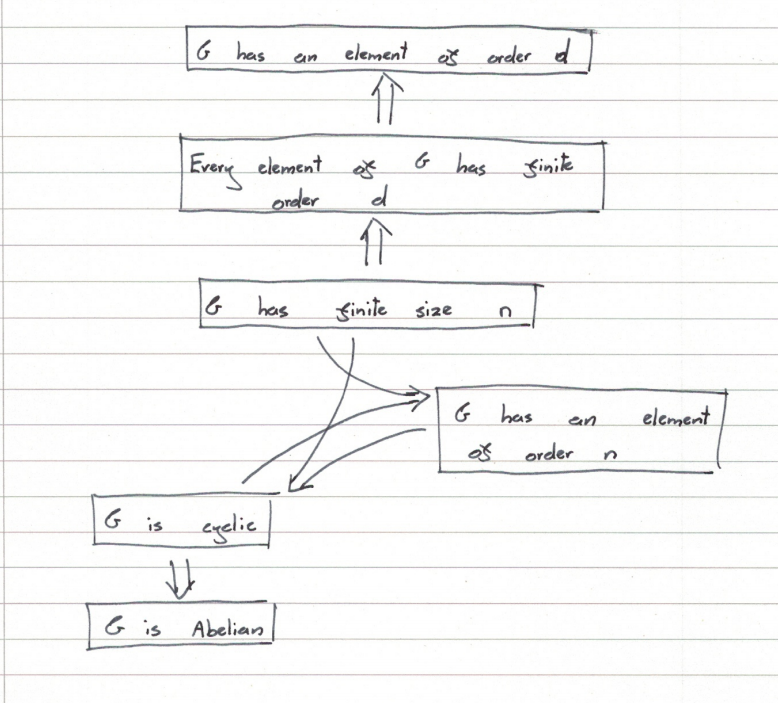
\includegraphics[scale=0.4]{cyclic_groups}

\subsection{Symmetric groups}
($ S_{n}, \circ $) is a group.
\\\\
The size of any $ S_{n} $ is $ n! $
\\\\
The order of a $ k $-cycle  is $ k $.
\\\\
For any $ \sigma \in S_{n} $:
\begin{itemize}
\item for any $ i \in \{0...n\} $ there exists a $ d  > 0 $ such that $ \sigma^{d}(i) = i $ (i.e. $ \sigma^{d} \equiv Id = e $)
\item if $ d $ is the smallest integer such that $ \sigma^{d}(i) = i $ then the numbers $ i, \sigma^{1}(i), \sigma^{2}(i) ... \sigma^{d - 1}(i) $ are distinct
\item If $ j $ is not in the set $ \{i, \sigma(i), \sigma^{2}(i)...\sigma^{d - 1}(i)\} $ then neither is $ \sigma(j) $
\end{itemize}
Any permutation $ \sigma $ can be expressed as the product of disjoint $ k $-cycles.

\subsection{Subgroups}
Any group ($ G, \star $) has two trivial subgroups, ($ e, \star $) and itself.
\\\\
\textit{Subgroup test}
\\
Any $ H \subseteq G $ is a subgroup if:
\begin{itemize}
\item $ H \neq \emptyset $
\item for all $ x, y \in H, x \star y^{-1} \in H $
\end{itemize}

\subsection{Cosets and Lagrange's Theorem}
For any $ g_{1}, g_{2} \in G $ and subgroup $ H $:
\begin{equation}
g_{1}H = g_{2}H \Leftrightarrow g_{1} \in g_{2}H
\end{equation}
The left cosets of $ H $ form a partition of $ G $. This means any $ g \in G $ is in exactly one left coset of $ H $. The right cosets also form a (different) partition.
\\\\
For any $ g \in G $:
\begin{equation}
\#gH = \#hG = \#H
\end{equation}
\\
\textit{Lagrange's Theorem}
\\
For any subgroup ($ H, \star $) where $ H \subseteq G $:
\begin{equation}
\#G = \#H \cdot \#(G : H)
\end{equation}
\\
For any subgroup ($ H, \star $), $ \#H $ divides $ \#G $. (Consequence of Lagrange's Theorem).
\\\\
For any $ g \in G $, the order of $ g $ divides $ \#G $. (Since the order of $ g $ is the size of the subgroup $ \langle g \rangle $).
\\\\
If $ \#G = p $, where $ p $ is prime, then $ G $ is cyclic.

\newpage
\part{Analysis}

\section{Definitions}
\paragraph{Sequence}
A sequence is simply a map $ f: \N \to \R $, denoted by $ a_{n} $
\paragraph{Convergence (as $ n \to \infty $)}
A sequence $ a_{n} $ converges to a limit L if for all real numbers $ \epsilon > 0 $, there exists an $ N \in \N $ such that for all $ n > N $ we have $ |a_{n} - L| < \epsilon $.
\begin{equation}
\forall \epsilon > 0 \quad \exists N \in \N \quad s.t \quad \forall n > N \quad |a_{n} - L| < \epsilon
\end{equation}
\paragraph{Tends to infinity (sequence)}
We say a sequence tends to infinity if for all $ R \in \R $, the sequence $ a_{n} $ is eventually bigger than $ R $.
\begin{equation}
\forall R \in \R \quad \exists N \in \N \quad s.t. \quad \forall n > N \quad a_{n} > R
\end{equation}
\paragraph{Shift}
The shift of a sequence by say, k, is the sequence $ b_{n} = a_{n + k} $
\paragraph{Triangle inequality}
The general triangle inequality is:
\begin{equation}
|x - y| < |x - z| + |z - y|
\end{equation}
Setting $ z = 0 $ gives us:
\begin{align}
|x - y| & > |x| - |y|
\end{align}
Then setting $ y = - y $ gives us the familiar case:
\begin{align}
|x + y| & < |x| + |y|
\end{align}
\paragraph{Bounded above}
A sequence $ a_{n} $ is bounded above if there's a real number $ A $ such that $ a_{n} < A $ for all $ n $.
\paragraph{Bounded below}
A sequence $ a_{n} $ is bounded below if there's a real number $ A $ such that $ a_{n} > A $ for all $ n $.
\paragraph{Bounded}
A sequence $ a_{n} $ is bounded if there's a real number $ A $ such that $ |a_{n}| < A $ for all $ n $.
\paragraph{Increasing}
A sequence is increasing if $ a_{n + 1} \geq a_{n} $ for all n.
\paragraph{Strictly increasing}
A sequence is strictly increasing if $ a_{n + 1} > a_{n} $ for all n.
\paragraph{Decreasing}
A sequence is decreasing if $ a_{n + 1} \leq a_{n} $ for all n.
\paragraph{Strictly decreasing}
A sequence is strictly decreasing if $ a_{n + 1} < a_{n} $ for all n.
\paragraph{Monotonic}
A sequence is monotonic if it is increasing or decreasing.
\paragraph{Supremum}
The supremum A of a set $ S $ is the least upper bound of that set i.e. the smallest number such that $ s \leq A $ for all $ s \in S $.
\paragraph{Supremum (function)}
The supremum of a function $ f $ is the sup of $ \{f(x) \ | \ x \in \textrm{dom}(f)\} $.
\paragraph{Infimum}
The infimum B of a set $ S $ is the greatest lower bound of that set i.e. the largest number such that $ s \geq B $ for all $ s \in S $.
\paragraph{Infimum (function)}
The infimum of a function $ f $ is the inf of $ \{f(x) \ | \ x \in \textrm{dom}(f)\} $.
\paragraph{Subsequence}
A subsequence of $ a_{n} $ is a sequence $ a_{f(n)} $, where $ f(n) $ is a strictly increasing function.
\paragraph{Cauchy sequence}
A sequence is Cauchy if all the terms get arbitrarily close to one another. To put it mathematically:
\begin{equation}
\forall \epsilon > 0 \quad \exists N \in \N \quad s.t \quad \forall m,n \geq N \quad |a_{n} - a_{m}| < \epsilon
\end{equation}
\paragraph{Partial sum}
The $ n^{th} $ partial sum $ S_{n} $ of a sequence $ a_{n} $ is the sum of terms up to that point:
\begin{equation}
S_{n} = \sum_{i=1}^{n} a_{n}
\end{equation}
\paragraph{Summable}
A sequence is summable if the sequence of its partial sums converges. The limit of the sequence of partial sums will be:
\begin{equation}
L = \sum_{i=1}^{\infty} a_{n}
\end{equation}
\paragraph{Absolutely summable}
A sequence $ a_{n} $ is absolutely summable if $ |a_{n}| $ is summable.
\paragraph{Conditionally summable}
A sequence is conditionally summable if it is summable but not absolutely summable.
\paragraph{Power series}
The power series associated with a sequence $ a_{n} $ is the sequence of partial sums:
\begin{equation}
\sum_{i=1}^{n} a_{i}x^{i}
\end{equation}
\paragraph{Radius of convergence}
The radius of convergence R of a power series $ P(x) $ is defined as the largest $ x $ for which $ P(x) $ is convergent.
\begin{equation}
R = sup\{x \in \R \ | \ P(x) \textrm{ convergent}\}
\end{equation}
\paragraph{Limit as $ x \to \infty $ (function)}
A function $ f(x) $ tends to a limit $ L $ as $ x \to \infty $ if for all real numbers $ \epsilon > 0 $, there exists an $ R \in \R $ such that for all $ x \geq R $ we have $ |f(x) - L| < \epsilon $.
\begin{equation}
\forall \epsilon > 0 \quad \exists R \in \R \quad s.t \quad \forall x > R \quad |f(x) - L| < \epsilon
\end{equation}
\paragraph{Tends to infinity (function)}
A function $ f(x) $ tends to infinity as $ x \to \infty $ if for any $ M \in \R $ there exists an $ R \in \R $ such that if $ x > M $ then $ f(x) > R $.
\begin{equation}
\forall M \in \R \quad \exists R \in \R \quad s.t. \quad x > M \Rightarrow f(x) > R
\end{equation}
\paragraph{One-sided limit}
A function $ f(x) $ tends to a limit $ L $ as $ x \to a^{-} $ if for any $ \epsilon > 0 $ there exists a $ \delta > 0 $ such that if $ x \in (a - \delta, a) $ then $ |f(x) - L| < \epsilon $.
\begin{equation}
\forall \epsilon > 0 \quad \exists \delta > 0 \quad s.t. \quad x \in (a - \delta, a) \Rightarrow |f(x) - L| < \epsilon
\end{equation}
\noindent Same format for the other sided limit ($ x \to a^{+} $)
\\
(Note that $ \epsilon - \delta $ definition is only used for limits as x tends to a finite number a, not infinity)
\paragraph{Limit as $ x \to a $}
A function $ f(x) $ tends to a limit $ L $ as $ x \to a $ if we have both:
\begin{equation}
\lim_{x \to a^{-}}f(x) = L \quad \textrm{and} \quad \lim_{x \to a^{+}}f(x) = L
\end{equation}
\paragraph{Limit as $ x \to a $ ($ \epsilon $ - $ \delta $ def.)}
A function $ f(x) $ tends to a limit $ L $ as $ x \to a $ if:
\begin{equation}
\forall \epsilon > 0 \quad \exists \delta > 0 \quad s.t. \quad |x - a| < \delta \Rightarrow |f(x) - L| < \epsilon
\end{equation}
\paragraph{Continuous}
A function $ f(x) $ is continuous at a if:
\begin{equation}
\lim_{x \to a}f(x) = f(a)
\end{equation}
\paragraph{Continuous ($ \epsilon $ - $ \delta $ def.)}
A function $ f(x) $ is continuous at a if for all $ \epsilon > 0 $ there is a $ \delta > 0 $ such that if $ |x - a| < \delta $ then $ |f(x) - f(a)| < \epsilon $.
\begin{equation}
\forall \epsilon > 0 \quad \exists \delta > 0 \quad s.t. \quad |x - a| < \delta \Rightarrow |f(x) - f(a)| < \epsilon
\end{equation}
\paragraph{Continuous everywhere}
A function $ f(x) $ is continuous everywhere if it is continuous at a for all $ a \in \textrm{dom}(f) $.
\paragraph{Open interval}
An open inteval $ I $ is a set $ I \subseteq \R $ of the form:
\begin{itemize}
\item $ I = (a, b) $ for some $ a, b \in \R $, or
\item $ I = (-\infty, b) $, or
\item $ I = (a, +\infty) $, or
\item $ I = \R $
\end{itemize}
\paragraph{Discontinuity}
Discontinuity is the negation of continuity. Hence a function $ f(x) $ is discontinuous at a if there exists $ \epsilon > 0 $ such that for all $ \delta > 0 $, $ |x - a| < \delta $ AND $ |f(x) - f(a)| > \epsilon $.
\begin{equation}
\exists \epsilon > 0 \quad s.t. \quad \forall \delta > 0 \quad |x - a| < \delta \textrm{ AND } |f(x) - f(a)| > \epsilon
\end{equation}
\paragraph{Bounded (function)}
A function $ f(x) $ is bounded if the set of all possible values of f(x) is bounded.
\paragraph{Differentiable (ver. 1)}
A function $ f(x) $ is differentiable at a if:
\begin{equation}
\lim_{x \to a}\frac{f(x) - f(a)}{x - a}
\end{equation}
exists.
\paragraph{Differentiable (ver. 2)}
A function $ f(x) $ is differentiable at a if:
\begin{equation}
\lim_{h \to 0}\frac{f(a + h) - f(a)}{h}
\end{equation}
exists.
\paragraph{Differentiable everywhere}
A function $ f(x) $ is differentiable everywhere if it is differentiable at a for all $ a \in \textrm{dom}(f) $.
\paragraph{Global maximum}
A function $ f(x) $ has a global maximum at a if $ f(a) \geq f(x) $ for all other values of $ f(x) $.
\\\\
Similar definition for global minimum.
\paragraph{Local maximum}
A function $ f(x) $ has a local maximum at a if $ f(a) \geq f(x) $ for all x in the set $ (a - \epsilon, a + \epsilon) $, for some $ \epsilon $.
\\\\
Similar definition for local minimum.
\paragraph{Lipschitz continuous}
A function is Lipschitz continuous if:
\begin{equation}
|f'(x)| \leq L \Rightarrow |f(x_{1}) - f(x_{2})| \leq L|x_{1} - x_{2}|
\end{equation}

\section{Theorems}
\subsection{Sequences}
Every convergent sequence has a unique limit.
\\\\
Every convergent sequence is bounded.
\\\\
If all terms of a convergent sequence are larger than a number $ B $, then so is its limit.
\\\\
Some properties of limits:
\begin{align}
\lim_{x \to \infty}(a_{n} + b_{n}) & = \lim_{x \to \infty} a_{n} + \lim_{x \to \infty} b_{n} \\
\lim_{x \to \infty}(\lambda a_{n}) & = \lambda\lim_{x \to \infty} a_{n} \\
\lim_{x \to \infty}(a_{n}b_{n}) & = \lim_{x \to \infty} a_{n}\lim_{x \to \infty} b_{n} \\
\lim_{x \to \infty}(\frac{a_{n}}{b_{n}}) & = \frac{\lim_{x \to \infty} a_{n}}{\lim_{x \to \infty} b_{n}}
\end{align}
where $ \lambda $ is any real number.
\\\\
If $ a_{n} \to \infty $ and $ b_{n} $ is bounded below, $ a_{n} + b_{n} \to \infty $.
\\\\
If $ a_{n} \to \infty $ and $ b_{n} $ is bounded below by a positive number, $ a_{n}b_{n} \to \infty $.
\\\\
If $ a_{n} $ is bounded and $ b_{n} \to \infty $, then $ \frac{a_{n}}{b_{n}} \to 0 $.
\\\\
If $ a_{n} \to \infty $, for any real number $ \lambda $:
\begin{itemize}
\item $ \lambda < 0 \Rightarrow \lambda a_{n} \to -\infty $
\item $ \lambda = 0 \Rightarrow \lambda a_{n} \to 0 $
\item $ \lambda > 0 \Rightarrow \lambda a_{n} \to \infty $
\end{itemize}
If $ a_{n} \to a $ and $ b_{n} \to b $, and for all $ n $ $ a_{n} < b_{n} $, then $ a < b $.
\\\\
\textit{Sandwich Theorem}
\\
If $ a_{n} \leq b_{n} \leq c_{n} $ for all n, and $ a_{n} $ and $ c_{n} $ tend to the same limit $ L $, then $ b_{n} \to L $.
\\\\
Every bounded monotonic sequence is convergent.
\\\\
\textit{Completeness Axiom}
\\
Every non-empty subset of the real numbers which is bounded above has a supremum. Corresponding statement for infimum.
\\\\
Useful results for sequences:
\begin{align}
\lim_{n \to \infty} \lambda^{n} = 
\begin{cases}
\infty & \lambda > 1 \\
1 & \lambda = 1 \\
0 & -1 < \lambda < 1
\end{cases}
\end{align}
\begin{center}
$ \lambda^{n} $ diverges if $ \lambda = -1 $.
\end{center}
\begin{center}
If $ m > 0 $ and $ \lambda > 1 $ then $ \frac{\lambda^{n}}{n^{m}} \to \infty $ (exponentials beat powers).
\end{center}
\begin{center}
If $ m > 0 $ then $ \frac{\log(n)}{n^{m}} \to 0 $ (powers beat logs).
\end{center}

\subsection{Subsequences}
If $ a_{n} \to L $ then any subsequence $ a_{f(n)} \to L $.
\\\\
If two subsequences of $ a_{n} $ converge to different limits, $ a_{n} $ doesn't converge to a limit.
\\\\
Every sequence has a monotonic subsequence.
\\\\
\textit{Bolzano-Weierstrass Theorem}
\\
Every bounded sequence has a convergent subsequence.
\\\\
Every Cauchy sequence is bounded.
\\\\
Cauchy sequence $ \Leftrightarrow $ convergent sequence (for real numbers).
\\\\
\hspace*{-1in}
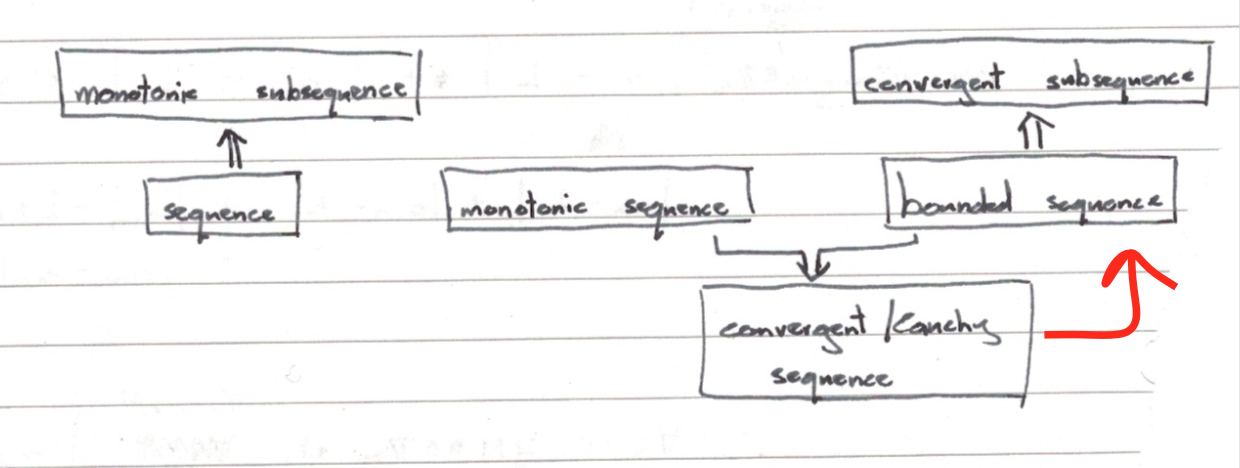
\includegraphics[scale=0.4]{sequences}

\subsection{Summability}
A sequence is summable iff the sequence of its partial sums converges.
\\\\
If two subsequences of a sequence $ a_{n} $ converge to two different limits, $ a_{n} $ is not summable.
\\\\
If $ a_{n} $ and $ b_{n} $ are summable with $ \sum_{i = 0}^{\infty} a_{i} = a $ and $ \sum_{i = 0}^{\infty} b_{i} = b $:
\begin{itemize}
\item $ a_{n} + b_{n} $ is summable with $ \sum_{i = 0}^{\infty} (a_{i} + b_{i}) = a + b $.
\item $ \lambda a_{n} $ is summable with $ \sum_{i = 0}^{\infty} \lambda a_{i} = \lambda a $ (for any real number $ \lambda $)
\end{itemize}
If $ b_{n} = a_{n + k} $ then $ a_{n} $ summable $ \Leftrightarrow b_{n} $ summable.
\\\\
$ a_{n} $ is summable $ \Rightarrow a_{n} \to 0 $.
\\\\
Let $ S_{n} $ denote the sequence of partial sums of $ a_{n} $ ($ S_{n} = \sum_{i = 0}^{n} a_{n}) $. A sequence of non-negative numbers $ a_{n} $ is summable iff $ S_{n} $ is bounded above. Similar statement for sequences of non-positive numbers.
\\\\
Every absolutely summable sequence is summable.
\\\\
\textit{Comparison test}
\\
If $ b_{n} > a_{n} $ for all $ n $ then $ b_{n} $ summable $ \Rightarrow a_{n} $ summable.
\\\\
\textit{Alternating series test}
\\
If $ a_{n} $ is a decreasing sequence AND $ a_{n} \geq 0 $ for all $ n $ AND $ a_{n} \to 0 $ then $ (-1)^{n+1} a_{n} $ is a convergent sequence.
\\\\
\textit{Ratio test for sequences}
\\
Let $ r = \lim_{n \to \infty} \frac{a_{n + 1}}{a_{n}} $:
\begin{itemize}
\item $ r < 1 \Rightarrow a_{n} $ is absolutely summable
\item $ r > 1 \Rightarrow a_{n} $ is not summable
\item $ r = 1 $ is an indeterminate case
\end{itemize}

\subsection{Power series}
The power series associated with a sequence $ a_{n} $ converges iff the sequence of partial sums  of $ a_{n}x^{n} $ converges (i.e. if $ \sum_{i = 0}^{n} a_{i}x^{i} $ converges).
\\\\
Let $ P(x) $ be a power series. If $ P(a) $ converges absolutely for some $ a $, then $ P(x) $ converges absolutely for all $ x $ such that $ |x| < |a| $
\\\\
Let $ R $ be the radius of convergence of $ P(x) $. For all real numbers $ a $:
\begin{itemize}
\item $ |a| < R \Rightarrow P(a) $ converges absolutely
\item $ |a| > R \Rightarrow P(a) $ diverges
\end{itemize}
\textit{Ratio test for power series}
\\
Let $ r = \frac{a_{n + 1}}{a_{n}} $. Let $ P(x) = \sum_{i = 0}^{n} a_{i}x^{i} $ (i.e. the power series associated with $ a_{n} $):
\begin{itemize}
\item $ r \to 0 \Rightarrow R = \infty $
\item $ r \to L $ for some $ L \Rightarrow R = \frac{1}{L} $
\item $ r \to \infty \Rightarrow R = 0 $
\end{itemize}
Note: if $ r = 1 $ here then $ R = 1 $. This is DIFFERENT to the ratio test for sequences, where $ r = 1 $ is an indeterminate case.

\subsection{Continuity}
The limit of a function at any specific point is unique.
\\\\
If functions $ f $ and $ g $ are continuous at a:
\begin{itemize}
\item $ (f + g) $ is continuous at a
\item $ fg $ is continuous at a
\item $ \frac{1}{f(x)} and \frac{1}{g(x)} $ are continuous at a
\item $ g \circ f $ is continuous at a
\end{itemize}
Any polynomial in $ \R $ is continuous
\\\\
Any rational function in $ \R $ is continuous
\\\\
\textit{Sequential continuity}
\\
A function $ f $ is continuous at $ a $ iff $ f(a_{n}) \to f(a) $ for all sequences $ a_{n} $ such that $ a_{n} \to a $.
\\\\
Any continuous function on a closed bounded interval is bounded.
\\\\
\textit{Intermediate Value Theorem}
\\
If $ f $ continuous and $ f(a) \leq f(b) $ for some $ a, b $, then there exists some $ c \in [a, b] $ such that $ f(a) \leq f(c) \leq f(b) $.
\\\\
\textit{Fixed Point Theorem}
\\
If $ f $ continuous and $ f: [a, b] \to [a, b] $, then there exists some $ c \in [a, b] $ such that $ f(c) = c $.
\\\\
Polynomials of odd degree have at least 1 root.
\\\\
$ f $ differentiable $ \Rightarrow f $ continuous.
\subsection{Differentiable functions}
If functions $ f $ and $ g $ are differentiable at a:
\begin{itemize}
\item $ (f + g) $ is differentiable at a
\item $ fg $ is differentiable at a
\item $ \frac{1}{f(x)} and \frac{1}{g(x)} $ are differentiable at a
\item $ g \circ f $ is differentiable at a
\item $ g^{-1} $ and $ f^{-1} $ are differentiable at a
\end{itemize}
Let $ f $ be continuous and differentiable. If $ f $ has a local extremum at $ a $ then $ f'(a) = 0 $ (except at endpoints of the interval).
\\\\
Let $ f $ be continuous and differentiable. If $ f $ has a local extremum at $ c $ (say in the interval $ [a, b] $), there are 3 possiblities:
\begin{itemize}
\item $ c $ is an endpoint of $ [a, b] $
\item $ f'(c) = 0 $
\item $ c $ is a non-differentiable point
\end{itemize}
\textit{Mean Value Theorem}
\\
Let $ f $ be continuous on $ [a, b] $ and differentiable on $ (a, b) $. There exists a point $ c \in (a, b) $ such that:
\begin{equation}
f'(c) = \frac{f(b) - f(a)}{b - a}
\end{equation}
\\\\
\textit{Rolle's Theorem}
\\
Let $ f $ be continuous and differentiable on $ (a, b) $. If $ f(a) = f(b) $ then there exists some $ c \in (a, b) $ such that $ f'(c) = 0 $. This is a special case of the Mean Value Theorem.

\end{document}